\documentclass[12pt,letterpaper]{article}

\usepackage[utf8]{inputenc}
\usepackage[T1]{fontenc}
\usepackage[spanish,es-nodecimaldot]{babel}
\usepackage{geometry}
\usepackage{graphicx}
\usepackage{booktabs}
\usepackage{longtable}
\usepackage{array}
\usepackage{tabularx}
\usepackage{amsmath}
\usepackage{amssymb}
\usepackage{xcolor}
\usepackage{hyperref}
\usepackage{microtype}
\Urlmuskip=0mu plus 1mu\relax

\geometry{top=2.4cm,bottom=2.4cm,left=2.7cm,right=2.7cm}
\graphicspath{{../results/graficos/}}
\setlength{\parindent}{0pt}
\setlength{\parskip}{0.55em}
\renewcommand{\arraystretch}{1.18}
\newcolumntype{Y}{>{\raggedright\arraybackslash}X}
\newcolumntype{C}{>{\centering\arraybackslash}X}
\definecolor{azulues}{RGB}{22,62,108}
\hypersetup{
  colorlinks=true,
  linkcolor=azulues,
  citecolor=azulues,
  urlcolor=azulues,
  pdftitle={Laboratorio 2: Question Answering y RAG},
  pdfauthor={Josias Abner Rivas Fuentes y Elmer Edenilson Rosales Molina},
  pdfsubject={Informe técnico final}
}

\begin{document}

\hypersetup{pageanchor=false}
\begin{titlepage}
  \centering
  {\Large\bfseries Universidad de El Salvador\par}
  \vspace{0.3cm}
  {\large Facultad de Ingeniería y Arquitectura\par}
  {\large Escuela de Sistemas Informáticos\par}
  \vspace{0.8cm}
  {\large Curso de Especialización en Machine Learning\par}
  \vfill
  {\Huge\bfseries Laboratorio 2\par}
  \vspace{0.5cm}
  {\LARGE Question Answering y Retrieval-Augmented Generation\par}
  \vspace{0.25cm}
  {\Large sobre documentación académica de la Universidad de El Salvador\par}
  \vspace{1.2cm}
  {\large Informe técnico final\par}
  \vfill
  \begin{tabular}{rl}
    \textbf{Estudiantes:} & Josias Abner Rivas Fuentes\\
                          & Elmer Edenilson Rosales Molina\\[0.3cm]
    \textbf{Catedrático:} & Vladimir Dias\\
    \textbf{Fecha:}       & 14 de agosto de 2026
  \end{tabular}
  \vfill
  \href{https://github.com/abner-rivas/Laboratorio---ML.git}
       {github.com/abner-rivas/Laboratorio---ML}
\end{titlepage}

\hypersetup{pageanchor=true}
\pagenumbering{roman}

\begin{abstract}
Este laboratorio estudia Question Answering (QA) extractivo en español y su
integración con recuperación semántica sobre normativa de la Universidad de El
Salvador. El desarrollo parte de contextos breves, compara tres modelos BETO,
evalúa seis configuraciones de fragmentación y construye un índice FAISS con
embeddings normalizados. La configuración monodocumento final combina
BETO-SQAC, MPNet multilingüe, chunks de 800 caracteres, solapamiento cero y
Top-10. Sobre el documento de 62 páginas y diez preguntas obtuvo
Recall@10 y QA Accuracy de 60\,\%. La extensión multidocumento conserva esa
configuración y amplía el corpus a nueve PDF, 199 páginas y 765 chunks. En ella,
Document Recall@10 fue 93.75\,\%, Chunk Recall@10 56.25\,\% y QA Accuracy
sobre preguntas respondibles 25\,\%. La brecha entre etapas demuestra que
seleccionar el documento no garantiza localizar la evidencia ni extraer el
span correcto. Se preservan los resultados negativos, la procedencia de cada
fragmento y un análisis de errores por etapa.
\end{abstract}

\textbf{Palabras clave:} Question Answering, QA extractivo, BETO, RAG,
embeddings, MPNet, FAISS, recuperación semántica, chunking.

\tableofcontents
\listoffigures
\listoftables
\clearpage
\pagenumbering{arabic}

\section{Introducción}

Un sistema de Question Answering recibe una pregunta y un contexto, y busca
producir una respuesta sustentada en ese texto. En la variante extractiva, el
modelo predice las posiciones inicial y final de un span; no redacta una
respuesta nueva. BERT formalizó una arquitectura bidireccional de encoder que
puede ajustarse para esta tarea \cite{devlin2019}, mientras BETO adaptó esa
familia al español \cite{canete2020}.

La aplicación directa de QA a documentos extensos presenta dos problemas. Los
modelos evaluados admiten como máximo 512 tokens entre pregunta y contexto, y
la selección del mayor score entre cientos de fragmentos favorece falsos
positivos de alta confianza. El laboratorio aborda ambos problemas de manera
incremental: fragmenta el PDF, compara el coste de un barrido exhaustivo,
representa los chunks mediante embeddings y recupera únicamente los candidatos
mejor posicionados antes de ejecutar BETO-SQAC.

La denominación RAG se conserva por continuidad con el proyecto y con el
paradigma de recuperación aumentada \cite{lewis2020}; sin embargo, la etapa de
respuesta implementada es extractiva, no generativa. Esta precisión permite
interpretar correctamente el sistema y sus limitaciones.

\section{Objetivos}

\subsection{Objetivo general}

Diseñar y evaluar un sistema de preguntas y respuestas extractivo en español
sobre contextos breves y documentos institucionales extensos, incorporando
recuperación semántica y analizando por separado calidad de respuesta,
recuperación, procedencia y coste computacional.

\subsection{Objetivos específicos}

\begin{itemize}
  \item Comparar modelos QA en español bajo preguntas y criterios comunes.
  \item Extraer y fragmentar un PDF real sin perder offsets ni páginas.
  \item Evaluar tamaño de chunk, solapamiento, Top-K y modelo de embeddings.
  \item Construir una base vectorial exacta con FAISS.
  \item Distinguir score QA, Accuracy, Recall@K y MRR.
  \item Conservar el laboratorio monodocumento como experimento independiente.
  \item Extender el pipeline a varios PDF con metadata documental completa.
  \item Clasificar errores sin cambiar preguntas, etiquetas o respuestas.
\end{itemize}

\section{Fundamentos teóricos}

\subsection{Transformer, BERT y BETO}

El Transformer reemplaza recurrencia y convoluciones por mecanismos de
atención que relacionan los tokens de una secuencia \cite{vaswani2017}. BERT
usa un encoder bidireccional preentrenado y puede ajustarse para estimar logits
de inicio y fin de respuesta \cite{devlin2019}. BETO es un modelo BERT
preentrenado específicamente con texto en español \cite{canete2020}.

Los tres checkpoints evaluados pertenecen a esta familia. No se entrenaron
modelos desde cero ni se modificaron sus pesos; se ejecutó inferencia mediante
la interfaz de QA extractivo de Transformers \cite{huggingfaceqa}. El modelo
final es el checkpoint BETO-SQAC publicado por MMG \cite{mmgmodel}.

\subsection{Score y exactitud}

El score del pipeline mide la confianza relativa en un span dentro del
contexto recibido. No comprueba que el contexto sea pertinente y no equivale a
Accuracy. En el proyecto se etiquetaron scores altos desde 0.75, medios desde
0.40 y bajos por debajo de 0.40. Estos umbrales son operativos y no universales.

Para $N$ preguntas, la exactitud es
\begin{equation}
  \operatorname{Accuracy} =
  \frac{\text{respuestas correctas}}{N}.
  \label{eq:accuracy}
\end{equation}
La evaluación normaliza mayúsculas, diacríticos y signos; acepta igualdad,
presencia de la respuesta dentro de un span mayor y variantes explícitamente
declaradas. Las revisiones permanecen identificadas.

\subsection{Chunking y overlap}

El documento se divide en ventanas de longitud $L$ caracteres. Si el
solapamiento es $O$, el desplazamiento entre inicios consecutivos es
\begin{equation}
  P=L-O.
  \label{eq:paso}
\end{equation}
El overlap puede proteger evidencia cercana a un corte, pero aumenta
duplicación, número de chunks e inferencias. Su utilidad debe evaluarse en vez
de asumirse.

\subsection{Embeddings, coseno y FAISS}

Sentence-BERT produce representaciones densas adecuadas para similitud
semántica \cite{reimers2019}. El modelo final usa una variante multilingüe
basada en MPNet \cite{song2020,mpnetmodel}. Dados dos vectores $\mathbf{a}$ y
$\mathbf{b}$, la similitud coseno es
\begin{equation}
  \cos(\theta)=
  \frac{\mathbf{a}^{\mathsf T}\mathbf{b}}
       {\lVert\mathbf{a}\rVert_2\lVert\mathbf{b}\rVert_2}.
  \label{eq:coseno}
\end{equation}
Con normalización L2, el producto interno coincide con el coseno:
\begin{equation}
  \widehat{\mathbf a}^{\mathsf T}\widehat{\mathbf b}
  =\cos(\widehat{\mathbf a},\widehat{\mathbf b}).
\end{equation}
Por ello se usó FAISS \texttt{IndexFlatIP}, un índice exacto que conserva la
interpretabilidad del ranking \cite{johnson2019}. FAISS recupera contexto; no
genera ni evalúa la respuesta.

\subsection{Recall@K y MRR}

Recall@K mide la proporción de preguntas cuya evidencia aparece entre los $K$
primeros candidatos:
\begin{equation}
  \operatorname{Recall@K} =
  \frac{\text{preguntas con evidencia en Top-K}}
       {\text{preguntas evaluables}}.
  \label{eq:recall}
\end{equation}
El rango recíproco medio resume cuán pronto aparece el primer resultado
relevante:
\begin{equation}
  \operatorname{MRR} =
  \frac{1}{N}\sum_{i=1}^{N}\frac{1}{r_i},
  \label{eq:mrr}
\end{equation}
donde el término vale cero si la evidencia no aparece. En la extensión se
calculan rangos distintos para documento y chunk.

\section{Datos y preparación documental}

\subsection{Documento obligatorio}

La fuente de la parte obligatoria es el \emph{Reglamento de la Gestión
Académico-Administrativa de la Universidad de El Salvador}
\cite{uesreglamento}. PyMuPDF extrajo el texto página por página
\cite{pymupdfdocs}. No se aplicó OCR porque todas las páginas contenían texto.

\begin{table}[htbp]
  \centering
  \caption{Propiedades verificadas del documento obligatorio.}
  \label{tab:documento}
  \begin{tabular}{lr}
    \toprule
    Propiedad & Valor\\
    \midrule
    Páginas & 62\\
    Caracteres crudos & 177\,390\\
    Caracteres después de limpieza & 173\,419\\
    Palabras aproximadas & 26\,119\\
    Páginas con texto & 62\\
    Tamaño del PDF & 497\,732 bytes\\
    \bottomrule
  \end{tabular}
\end{table}

La limpieza eliminó guiones blandos, recompuso palabras separadas por salto de
línea y normalizó espacios. No resumió artículos ni corrigió el contenido. La
metadata conservó página, offsets y texto.

\subsection{Corpus multidocumento}

La extensión añade ocho reglamentos al PDF original sin concatenarlos. Cada
documento se extrae y fragmenta por separado; la concatenación ocurre solo a
nivel de la lista de metadata y de la matriz vectorial.

\begin{table}[htbp]
  \centering
  \caption{Alcance de los dos corpus ejecutados.}
  \label{tab:corpus}
  \begin{tabularx}{\textwidth}{YCC}
    \toprule
    Propiedad & Monodocumento & Multidocumento\\
    \midrule
    Documentos & 1 & 9\\
    Páginas & 62 & 199\\
    Palabras aproximadas & 26\,119 & 94\,263\\
    Chunks/vectores & 217 & 765\\
    Dimensión final & 768 & 768\\
    \bottomrule
  \end{tabularx}
\end{table}

Cada chunk multidocumento conserva \texttt{documento}, \texttt{pagina},
\texttt{chunk\_id}, identificador global, posición vectorial y \texttt{texto}.
La validación exige correspondencia uno a uno entre
\texttt{vector\_posicion}, metadata e índice FAISS.

\section{Metodología y arquitectura}

\subsection{Flujo monodocumento}

\begin{verbatim}
documento_fuente.pdf
  -> extracción y limpieza
  -> chunking 800/0
  -> embeddings MPNet normalizados
  -> FAISS IndexFlatIP, Top-10
  -> BETO-SQAC
  -> respuesta y evaluación
\end{verbatim}

Las diez preguntas documentales se anotaron con respuesta, artículo, página y
evidencia. El laboratorio no cambió preguntas ni respuestas esperadas para
mejorar resultados.

\subsection{Flujo multidocumento}

\begin{verbatim}
pregunta
  -> MPNet
  -> FAISS Top-10
  -> documento + página + chunk
  -> BETO-SQAC
  -> respuesta + score + fuente
\end{verbatim}

Las 18 preguntas incluyen 16 respondibles distribuidas entre los nueve PDF y
dos sin respuesta. Estas últimas no participan en Recall o MRR, pero sí en la
evaluación de abstención.

\subsection{Criterios de selección}

Las decisiones priorizaron respuestas correctas, recuperación y trazabilidad
antes que score o diferencias marginales de tiempo. Los tiempos proceden de
una ejecución por configuración. La semilla 42 controla la construcción
anidada de bases con distractores, pero no hace deterministas las mediciones.

\section{Comparación de modelos QA}

Se evaluaron tres checkpoints con cinco preguntas en cada uno de tres
contextos: UES, bases de datos y Wikipedia adaptada. La comparación controlada
final consta de 45 inferencias.

\begin{table}[htbp]
  \centering
  \caption{Comparación controlada y selección del extractor.}
  \label{tab:modelos}
  \small
  \begin{tabularx}{\textwidth}{Yrrrr}
    \toprule
    Modelo & Correctas & Accuracy & Score medio & Tiempo medio (s)\\
    \midrule
    BETO-SQuAD2 (mrm8488) & 13/15 & 86.67\,\% & 0.541198 & 0.1215\\
    BETO-SQuAD2 (MMG) & 13/15 & 86.67\,\% & 0.424900 & 0.1132\\
    BETO-SQAC (MMG) & 15/15 & 100\,\% & 0.691953 & 0.1154\\
    \bottomrule
  \end{tabularx}
\end{table}

BETO-SQAC fue el único modelo con 15/15 y se seleccionó como extractor. La
Figura~\ref{fig:modelos} corresponde al contexto inicial; apoya la comparación
de score y tiempo, pero no sustituye el agregado de la
Tabla~\ref{tab:modelos}.

\begin{figure}[htbp]
  \centering
  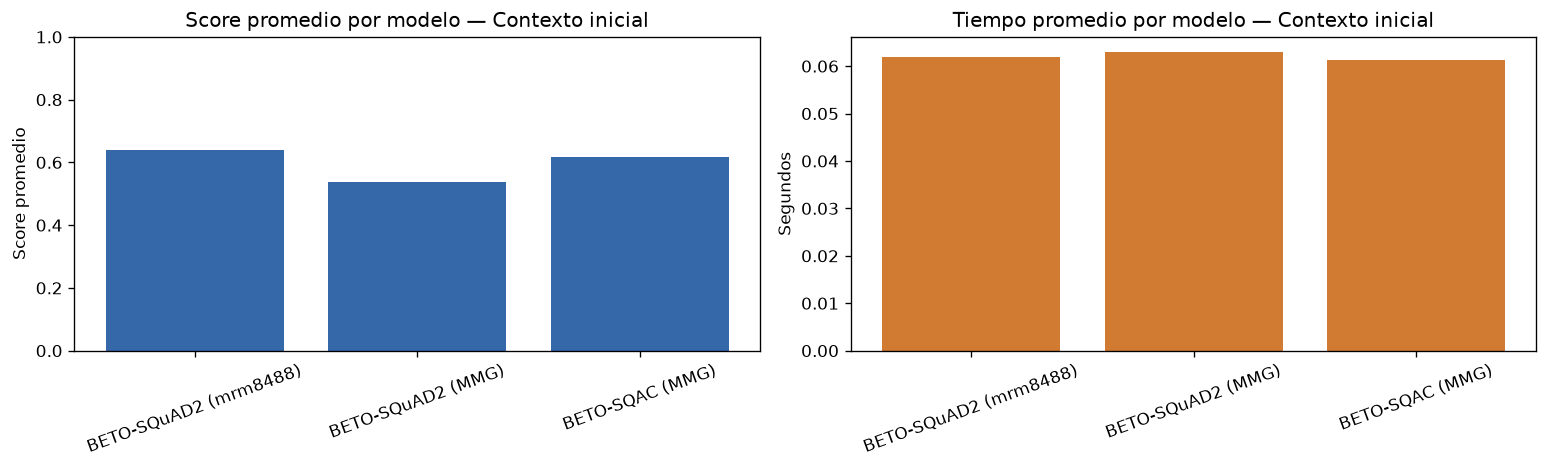
\includegraphics[width=0.92\textwidth]{../results/graficos/comparacion_modelos.png}
  \caption{Score y tiempo de los modelos en el contexto inicial. Fuente:
  resultados ejecutados del proyecto.}
  \label{fig:modelos}
\end{figure}

El archivo \path{results/comparacion_modelos.csv} conserva además un
benchmark histórico de 60 inferencias. La selección 13/15, 13/15 y 15/15 se
sustenta en \path{results/resultados_qa.csv}; ambos conjuntos se conservan y
no se mezclan.

\section{Fragmentación del documento}

Se evaluaron seis configuraciones, expresadas como tamaño/overlap en
caracteres.

\begin{table}[htbp]
  \centering
  \caption{Resultados de chunking y solapamiento.}
  \label{tab:chunking}
  \small
  \begin{tabular}{lrrrrr}
    \toprule
    Config. & Chunks & Correctas & Accuracy & Score medio & Tiempo (s)\\
    \midrule
    300/0   & 579 & 3/10 & 30\,\% & 0.935121 & 288.147\\
    300/50  & 694 & 4/10 & 40\,\% & 0.915775 & 350.798\\
    500/0   & 347 & 3/10 & 30\,\% & 0.917160 & 223.805\\
    500/100 & 434 & 4/10 & 40\,\% & 0.938941 & 325.274\\
    800/0   & 217 & 4/10 & 40\,\% & 0.942767 & 236.143\\
    800/150 & 267 & 4/10 & 40\,\% & 0.898146 & 282.039\\
    \bottomrule
  \end{tabular}
\end{table}

El overlap añadió un acierto en 300/50 y 500/100, pero no en 800/150; siempre
aumentó chunks y tiempo. Entre las configuraciones con 4/10, 800/0 tuvo la base
más pequeña, el menor tiempo y el mayor score medio. Se seleccionó como mejor
compromiso del conjunto evaluado, no como valor universal.

\section{Embeddings, FAISS y Top-K}

El primer RAG usó MiniLM multilingüe, 217 vectores de 384 dimensiones y los
mismos chunks 800/0. Se evaluaron $K=1,3,5,10$ sin reconstruir el índice.

\begin{table}[htbp]
  \centering
  \caption{Evaluación histórica de Top-K con MiniLM.}
  \label{tab:topk}
  \begin{tabular}{rrrrrr}
    \toprule
    K & Correctas & Accuracy & Recall@K & Score QA & Tiempo (s)\\
    \midrule
    1  & 1/10 & 10\,\% & 10\,\% & 0.269381 & 0.189\\
    3  & 3/10 & 30\,\% & 30\,\% & 0.640720 & 0.508\\
    5  & 3/10 & 30\,\% & 30\,\% & 0.702736 & 0.721\\
    10 & 4/10 & 40\,\% & 40\,\% & 0.836432 & 1.408\\
    \bottomrule
  \end{tabular}
\end{table}

Top-10 fue el único valor con cuatro respuestas correctas y se mantuvo en las
fases posteriores. La Figura~\ref{fig:topk} muestra el aumento de Accuracy; el
coste creció porque BETO recibió más contextos.

\begin{figure}[htbp]
  \centering
  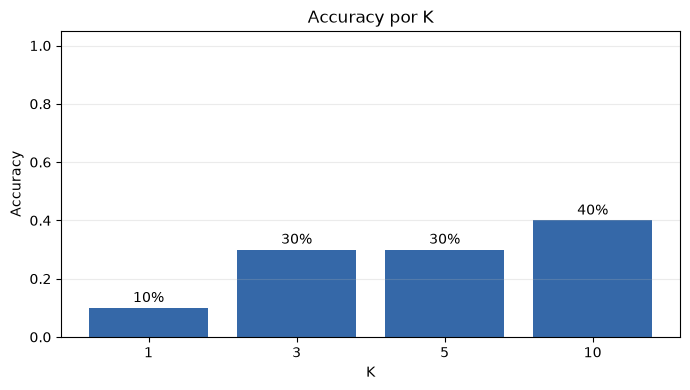
\includegraphics[width=0.78\textwidth]{../results/graficos/accuracy_topk.png}
  \caption{Accuracy histórica del RAG MiniLM para los cuatro valores de K.}
  \label{fig:topk}
\end{figure}

\section{Baseline exhaustivo frente a RAG}

\begin{table}[htbp]
  \centering
  \caption{Comparación histórica del barrido exhaustivo y RAG MiniLM.}
  \label{tab:baseline}
  \small
  \begin{tabularx}{\textwidth}{Yrrrr}
    \toprule
    Método & Correctas & Accuracy & Tiempo (s) & Inferencias QA\\
    \midrule
    QA exhaustivo 800/0 & 4/10 & 40\,\% & 236.143 & 2\,170\\
    RAG MiniLM Top-10 & 4/10 & 40\,\% & 1.408 & 100\\
    \bottomrule
  \end{tabularx}
\end{table}

El RAG redujo las inferencias en 95.4\,\% sin cambiar la Accuracy histórica. El
speedup registrado fue $167.75\times$, pero el baseline quedó en CPU y el RAG
posterior en CUDA. Por ello la Figura~\ref{fig:tiempo} se interpreta como
tiempo observado, no como aislamiento causal del aporte de FAISS.

\begin{figure}[htbp]
  \centering
  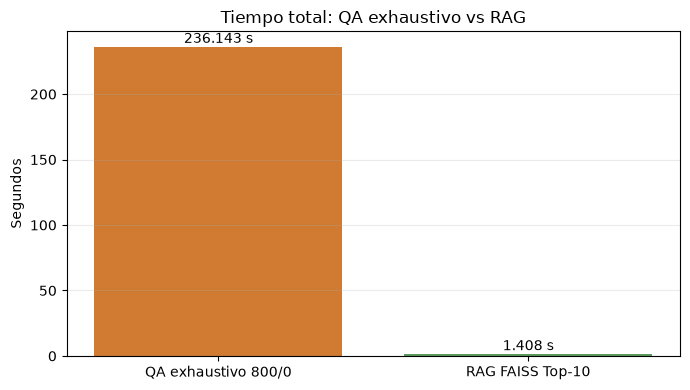
\includegraphics[width=0.78\textwidth]{../results/graficos/baseline_rag_tiempo.png}
  \caption{Tiempo registrado del baseline y RAG; las fases usaron dispositivos
  distintos.}
  \label{fig:tiempo}
\end{figure}

\section{Selección de embeddings y tamaño de base}

\subsection{MiniLM frente a MPNet}

\begin{table}[htbp]
  \centering
  \caption{Comparación controlada de embeddings.}
  \label{tab:embeddings}
  \small
  \begin{tabular}{lrrrrr}
    \toprule
    Modelo & Dim. & Recall@10 & Accuracy & Embeddings (s) & Consultas (s)\\
    \midrule
    MiniLM & 384 & 40\,\% & 40\,\% & 0.536 & 1.432\\
    MPNet & 768 & 60\,\% & 60\,\% & 1.642 & 1.420\\
    \bottomrule
  \end{tabular}
\end{table}

MPNet elevó Recall@10 y Accuracy en 20 puntos porcentuales. Sus embeddings
tardaron 3.06 veces más, pero el tiempo de consulta fue similar. La mejora se
atribuye al modelo completo bajo condiciones fijas, no únicamente a su
dimensión.

\begin{figure}[htbp]
  \centering
  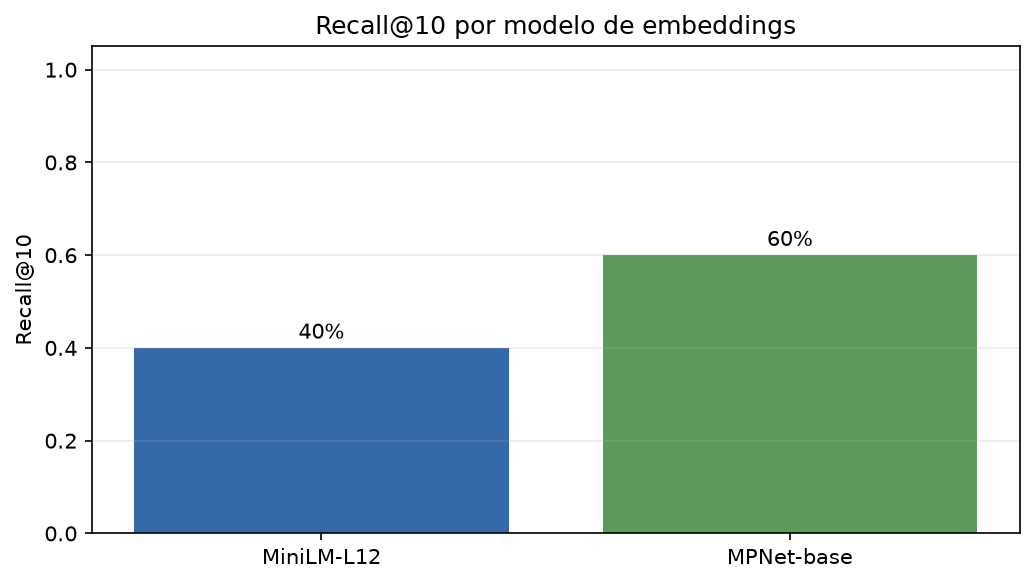
\includegraphics[width=0.9\textwidth]{../results/graficos/comparacion_embeddings_recall.png}
  \caption{Recall@10 con MiniLM y MPNet sobre los mismos 217 chunks.}
  \label{fig:embeddings}
\end{figure}

\subsection{Tamaño de la base vectorial}

Las bases de 50, 100, 150 y 217 vectores fueron anidadas y conservaron 11
chunks obligatorios con evidencia. Los restantes fueron distractores elegidos
con semilla 42.

\begin{table}[htbp]
  \centering
  \caption{Efecto de distractores con MPNet y Top-10.}
  \label{tab:tamano}
  \begin{tabular}{rrrrr}
    \toprule
    Vectores & Distractores & Recall@10 & Accuracy & Consultas (s)\\
    \midrule
    50  & 39  & 70\,\% & 50\,\% & 1.408\\
    100 & 89  & 70\,\% & 60\,\% & 1.410\\
    150 & 139 & 60\,\% & 60\,\% & 1.403\\
    217 & 206 & 60\,\% & 60\,\% & 1.412\\
    \bottomrule
  \end{tabular}
\end{table}

\begin{figure}[htbp]
  \centering
  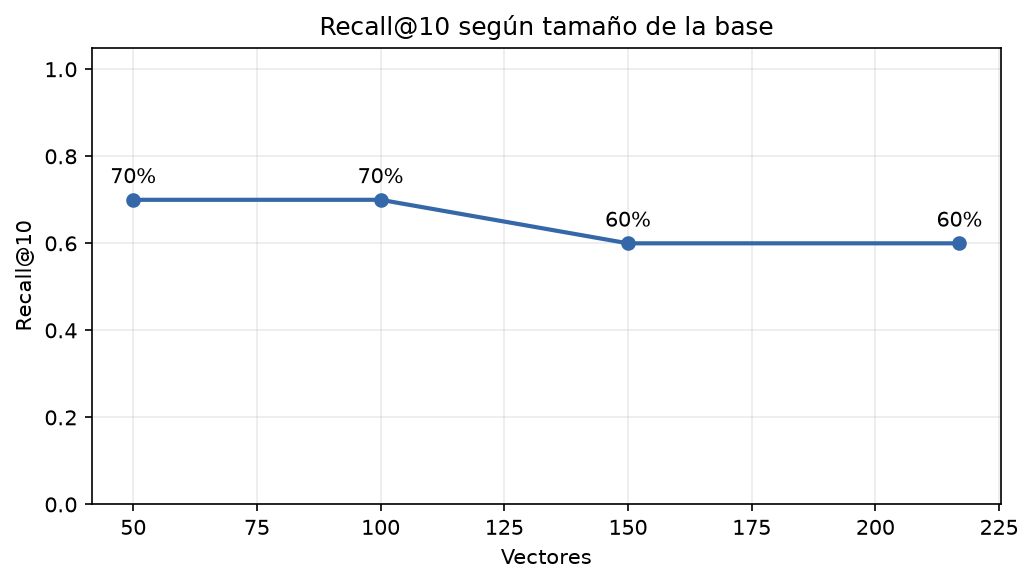
\includegraphics[width=0.9\textwidth]{../results/graficos/tamano_base_recall.png}
  \caption{Recall@10 según el tamaño controlado de la base.}
  \label{fig:tamano}
\end{figure}

La caída de Recall al agregar distractores no se debió a eliminar conocimiento:
la evidencia permaneció indexada, pero perdió posiciones. El tiempo fue casi
constante porque BETO procesó como máximo diez chunks en todos los tamaños.

\section{RAG monodocumento final}

\begin{table}[htbp]
  \centering
  \caption{Configuración final del laboratorio obligatorio.}
  \label{tab:configfinal}
  \begin{tabularx}{0.88\textwidth}{YY}
    \toprule
    Componente & Selección\\
    \midrule
    Documento & Reglamento académico-administrativo de la UES\\
    Modelo QA & BETO-SQAC (MMG)\\
    Embeddings & MPNet multilingüe\\
    Chunk / overlap & 800 / 0 caracteres\\
    Índice & FAISS \texttt{IndexFlatIP}\\
    Base & 217 vectores de 768 dimensiones\\
    Recuperación & Top-10; Recall@10 de 60\,\%\\
    Resultado & 6/10; QA Accuracy de 60\,\%\\
    \bottomrule
  \end{tabularx}
\end{table}

Esta configuración es la conclusión del experimento obligatorio. No se
recalcularon sus diez preguntas sobre el corpus ampliado ni se sustituyó el PDF
por un documento concatenado.

\section{Extensión RAG multidocumento}

\subsection{Diseño}

La extensión mantiene BETO-SQAC, MPNet, 800/0, \texttt{IndexFlatIP} y Top-10.
La base crece a 765 vectores, y la procedencia se convierte en variable
experimental. MPNet generó los embeddings en 6.147 s sobre CUDA y la matriz
\texttt{float32} ocupó 2.24 MiB.

\subsection{Resultados de recuperación}

\begin{table}[htbp]
  \centering
  \caption{Recuperación multidocumento por nivel y K.}
  \label{tab:multi-recall}
  \begin{tabular}{lrrrr}
    \toprule
    Métrica & K=1 & K=3 & K=5 & K=10\\
    \midrule
    Document Recall & 68.75\,\% & 87.50\,\% & 93.75\,\% & 93.75\,\%\\
    Chunk Recall & 25.00\,\% & 31.25\,\% & 43.75\,\% & 56.25\,\%\\
    \bottomrule
  \end{tabular}
\end{table}

Document Accuracy@1 fue 68.75\,\%; MRR documental, 0.7833; y MRR de chunk,
0.31875. Las Figuras~\ref{fig:docrecall} y~\ref{fig:chunkrecall} muestran la
brecha entre localizar un PDF relacionado y recuperar la evidencia exacta.

\begin{figure}[htbp]
  \centering
  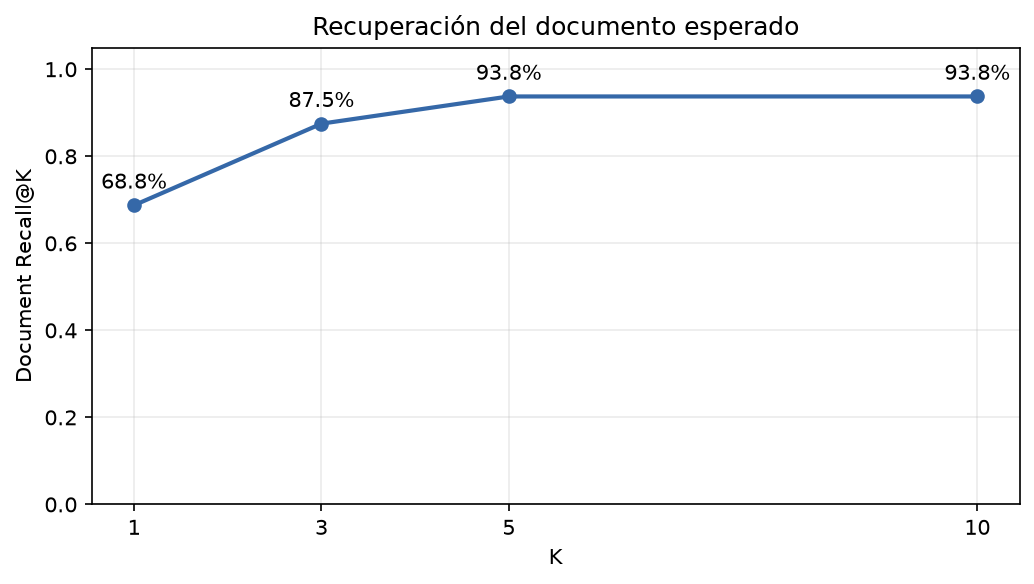
\includegraphics[width=0.88\textwidth]{../results/graficos/rag_multidocumento_document_recall_at_k.png}
  \caption{Document Recall@K de la extensión multidocumento.}
  \label{fig:docrecall}
\end{figure}

\begin{figure}[htbp]
  \centering
  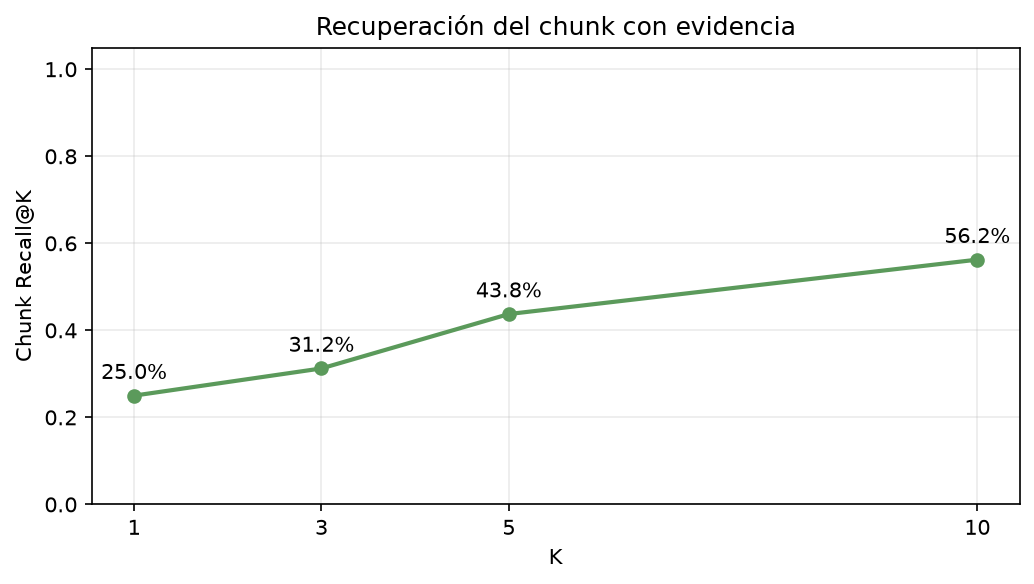
\includegraphics[width=0.88\textwidth]{../results/graficos/rag_multidocumento_chunk_recall_at_k.png}
  \caption{Chunk Recall@K: recuperación de página y evidencia anotadas.}
  \label{fig:chunkrecall}
\end{figure}

\subsection{Respuesta y abstención}

BETO-SQAC respondió correctamente 4 de 16 preguntas respondibles
(25\,\%) y 4 de 18 en total (22.22\,\%). Ninguna de las dos preguntas sin
evidencia produjo abstención; los spans fueron \texttt{sta} y \texttt{***}.

El comportamiento principal es una pérdida encadenada:
\begin{center}
  \large
  \textbf{93.75\,\char37\ Document Recall@10}
  $\longrightarrow$
  \textbf{56.25\,\char37\ Chunk Recall@10}
  $\longrightarrow$
  \textbf{25\,\char37\ QA Accuracy}
\end{center}
El sistema identifica casi siempre el documento relevante, pero eso no
garantiza el fragmento exacto. Después existe una pérdida adicional en QA.
Este resultado no se oculta ni se ajusta con nuevas etiquetas.

\section{Análisis de errores}

\subsection{Taxonomía}

La extensión usa categorías mutuamente excluyentes:

\begin{itemize}
  \item \textbf{Tipo A}: documento del candidato QA incorrecto.
  \item \textbf{Tipo B}: documento correcto, pero chunk ganador incorrecto.
  \item \textbf{Tipo C}: evidencia recuperada y QA incorrecto.
  \item \textbf{Tipo D}: respuesta parcialmente correcta.
  \item \textbf{Tipo E}: pregunta sin respuesta.
\end{itemize}

\begin{table}[htbp]
  \centering
  \caption{Errores observados en la extensión.}
  \label{tab:errores}
  \begin{tabular}{lr}
    \toprule
    Categoría & Casos\\
    \midrule
    A. Documento incorrecto & 6\\
    B. Documento correcto, chunk incorrecto & 6\\
    C. Recuperación correcta, QA incorrecto & 1\\
    D. Respuesta parcial & 0\\
    E. Pregunta sin respuesta & 2\\
    Sin error integral & 3\\
    \bottomrule
  \end{tabular}
\end{table}

Un caso informativo produjo el texto correcto «una vez al mes», pero desde la
Ley Orgánica y no desde el documento esperado. Sin metadata, ese falso positivo
documental habría sido contado como éxito integral. Los 18 registros, incluidos
los casos sin error, están en
\texttt{results/rag\_multidocumento\_errores.csv}.

\section{Discusión}

\subsection{Monodocumento frente a multidocumento}

\begin{table}[htbp]
  \centering
  \caption{Comparación descriptiva de los dos experimentos.}
  \label{tab:comparacion}
  \begin{tabularx}{\textwidth}{YCC}
    \toprule
    Característica & Monodocumento & Multidocumento\\
    \midrule
    Documentos & 1 & 9\\
    Páginas & 62 & 199\\
    Chunks & 217 & 765\\
    Recall@10 de evidencia & 60\,\% & 56.25\,\%\\
    QA Accuracy respondible & 60\,\% & 25\,\%\\
    Selección documental & No aplica & Sí\\
    Preguntas & 10 & 16 respondibles + 2 sin respuesta\\
    \bottomrule
  \end{tabularx}
\end{table}

Las métricas no deben compararse como si provinieran del mismo dataset. La
extensión usa preguntas nuevas, fuentes relacionadas y ambigüedad documental.
La Figura~\ref{fig:mono-multi} es descriptiva: muestra el coste experimental de
añadir fuentes, no una comparación pareada.

\begin{figure}[htbp]
  \centering
  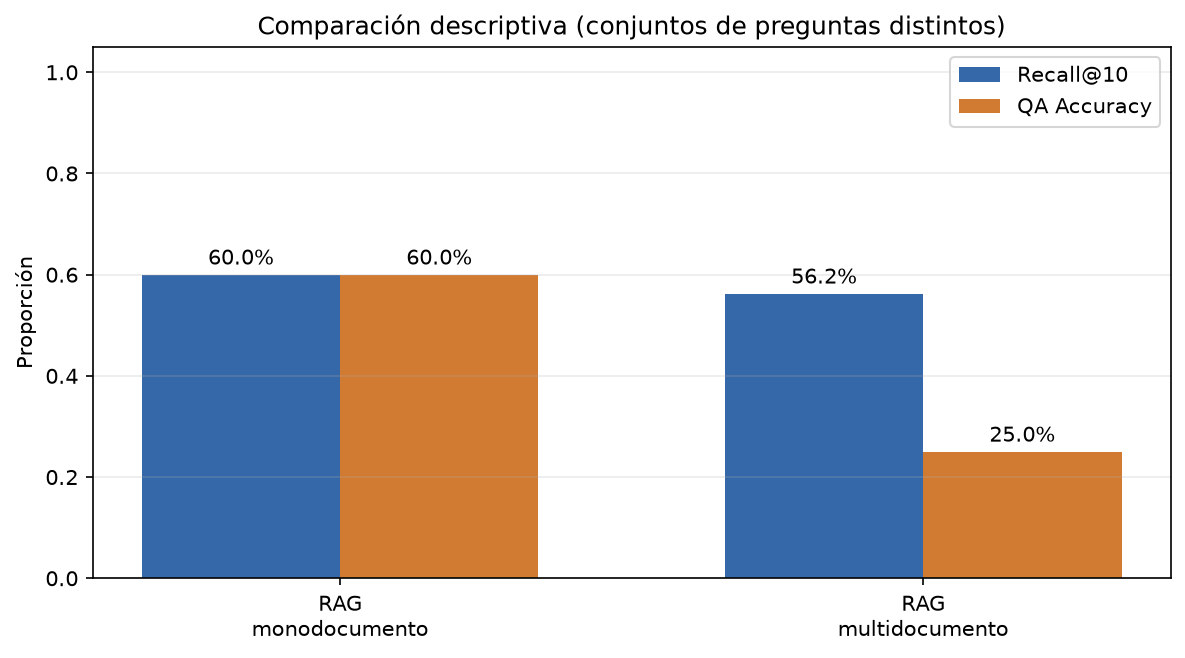
\includegraphics[width=0.88\textwidth]{../results/graficos/rag_monodocumento_vs_multidocumento.png}
  \caption{Comparación descriptiva; los conjuntos de preguntas son distintos.}
  \label{fig:mono-multi}
\end{figure}

\subsection{Decisiones técnicas}

\begin{itemize}
  \item \textbf{BETO-SQAC}: fue el único extractor con 15/15 en la comparación
  controlada.
  \item \textbf{MPNet}: mejoró Recall@10 y Accuracy de 40\,\% a 60\,\% frente a
  MiniLM bajo condiciones fijas.
  \item \textbf{FAISS}: permitió búsqueda exacta e interpretable a esta escala.
  \item \textbf{800/0}: empató en aciertos con menos chunks y menor coste entre
  las variantes de cuatro respuestas correctas.
  \item \textbf{Top-10}: fue el único K probado que alcanzó 4/10 con MiniLM.
\end{itemize}

Estas razones se basan en resultados ejecutados y no en ventajas inventadas a
posteriori.

\section{Limitaciones}

\begin{itemize}
  \item Diez preguntas finales en el experimento obligatorio y dieciocho en la
  extensión; cada caso representa varios puntos porcentuales.
  \item Una medición temporal por configuración y hardware diferente entre
  algunas fases históricas.
  \item Chunking fijo por caracteres, incapaz de integrar evidencia repartida
  entre ventanas.
  \item Dos modelos de embeddings, un índice exacto y ausencia de reranking.
  \item Umbral de abstención no calibrado para el dominio.
  \item Dependencias y revisiones de checkpoints no fijadas con certeza durante
  las ejecuciones originales.
  \item Corpus institucional de un solo dominio; no se evaluaron PDF escaneados
  ni colecciones de gran escala.
\end{itemize}

\section{Trabajo futuro}

Las extensiones no implementadas incluyen reranking; búsqueda híbrida con BM25;
chunking por artículo u overlap adaptativo; unión de chunks adyacentes; filtros
por metadata; y calibración de abstención. También quedan para otro estudio la
evaluación humana, más preguntas y mediciones repetidas sobre el mismo hardware.
Son nuevos experimentos, no resultados actuales.

\section{Reproducibilidad}

El notebook canónico conserva 273 celdas: 129 de código y 144 Markdown. Todas
tienen \texttt{execution\_count}, no existen salidas de error, tracebacks ni
celdas vacías. El notebook histórico se conserva únicamente como antecedente.

La ejecución ligera desde la raíz es:
\begin{verbatim}
python -m venv .venv
source .venv/bin/activate
python -m pip install -r requirements.txt
pytest -q
python -m unittest
python scripts/validar_entrega.py
python -m compileall src
\end{verbatim}

La reproducción completa mediante \emph{Run All} descarga modelos y repite
experimentos pesados. Para revisar la entrega no es necesaria: los CSV, la
metadata, el índice, los gráficos y las salidas del notebook ya están
conservados. La ejecución multidocumento registró Python 3.12.3, PyTorch
2.12.1+cu130, CUDA y semilla 42. No se creó un lock artificial porque no se
conocen con certeza todas las versiones originales.

La jerarquía de evidencia es: salidas finales del notebook; CSV específico del
experimento; código de apoyo; documentación narrativa. La auditoría automática
recalcula conteos y comprueba rutas sin ejecutar modelos.

\section{Conclusiones}

\begin{enumerate}
  \item BETO-SQAC fue el mejor extractor de los tres evaluados y obtuvo 15/15
  en la comparación controlada.
  \item La configuración 800/0 ofreció el mejor compromiso del barrido de
  chunking; el overlap no produjo una mejora uniforme.
  \item Top-10 mejoró la cobertura frente a K menores, a costa de más
  inferencias.
  \item MPNet elevó Recall@10 y Accuracy monodocumento a 60\,\%.
  \item FAISS redujo de 2\,170 a 100 las inferencias QA del contraste histórico.
  \item El score QA no sustituyó la evaluación: el baseline obtuvo 0.942767 de
  score medio con solo 40\,\% de Accuracy.
  \item En el corpus multidocumento, 93.75\,\% de Document Recall@10 cayó a
  56.25\,\% de Chunk Recall@10 y 25\,\% de QA Accuracy.
  \item La metadata documental fue necesaria para detectar respuestas
  textualmente correctas obtenidas desde una fuente equivocada.
  \item Las dos preguntas sin respuesta evidenciaron que el extractor requiere
  una regla de abstención externa y calibrada.
  \item Los resultados negativos se conservan como hallazgo experimental y no
  se modificaron para mejorar las métricas.
\end{enumerate}

\clearpage
\section*{Referencias}
\addcontentsline{toc}{section}{Referencias}

\begin{thebibliography}{99}

\bibitem{vaswani2017}
A. Vaswani, N. Shazeer, N. Parmar, J. Uszkoreit, L. Jones, A. N. Gomez,
{\L}. Kaiser e I. Polosukhin.
\newblock ``Attention Is All You Need''.
\newblock \emph{Advances in Neural Information Processing Systems 30}, 2017.
\newblock \url{https://proceedings.neurips.cc/paper/2017/hash/3f5ee243547dee91fbd053c1c4a845aa-Abstract.html}.

\bibitem{devlin2019}
J. Devlin, M.-W. Chang, K. Lee y K. Toutanova.
\newblock ``BERT: Pre-training of Deep Bidirectional Transformers for Language
Understanding''.
\newblock \emph{NAACL-HLT}, pp. 4171--4186, 2019.
\newblock DOI: \href{https://doi.org/10.18653/v1/N19-1423}{10.18653/v1/N19-1423}.

\bibitem{canete2020}
J. Cañete, G. Chaperon, R. Fuentes, J.-H. Ho, H. Kang y J. Pérez.
\newblock ``Spanish Pre-Trained BERT Model and Evaluation Data''.
\newblock \emph{Practical ML for Developing Countries Workshop, ICLR}, 2020.
\newblock \url{https://pml4dc.github.io/iclr2020/program/pml4dc_10.html}.

\bibitem{reimers2019}
N. Reimers e I. Gurevych.
\newblock ``Sentence-BERT: Sentence Embeddings using Siamese BERT-Networks''.
\newblock \emph{EMNLP-IJCNLP}, pp. 3982--3992, 2019.
\newblock DOI: \href{https://doi.org/10.18653/v1/D19-1410}{10.18653/v1/D19-1410}.

\bibitem{song2020}
K. Song, X. Tan, T. Qin, J. Lu y T.-Y. Liu.
\newblock ``MPNet: Masked and Permuted Pre-training for Language Understanding''.
\newblock \emph{Advances in Neural Information Processing Systems 33}, 2020.
\newblock \url{https://proceedings.neurips.cc/paper/2020/hash/c3a690be93aa602ee2dc0ccab5b7b67e-Abstract.html}.

\bibitem{johnson2019}
J. Johnson, M. Douze y H. Jégou.
\newblock ``Billion-scale similarity search with GPUs''.
\newblock \emph{IEEE Transactions on Big Data}, 7(3):535--547, 2019.
\newblock \url{https://arxiv.org/abs/1702.08734}.

\bibitem{lewis2020}
P. Lewis et al.
\newblock ``Retrieval-Augmented Generation for Knowledge-Intensive NLP Tasks''.
\newblock \emph{Advances in Neural Information Processing Systems 33}, 2020.
\newblock \url{https://proceedings.neurips.cc/paper/2020/hash/6b493230-Abstract.html}.

\bibitem{huggingfaceqa}
Hugging Face.
\newblock ``Question answering''.
\newblock Documentación oficial de Transformers.
\newblock \url{https://huggingface.co/docs/transformers/tasks/question_answering}.

\bibitem{mmgmodel}
MMG.
\newblock ``bert-base-spanish-wwm-cased-finetuned-sqac''.
\newblock Ficha del checkpoint.
\newblock \url{https://huggingface.co/MMG/bert-base-spanish-wwm-cased-finetuned-sqac}.

\bibitem{mpnetmodel}
Sentence Transformers.
\newblock ``paraphrase-multilingual-mpnet-base-v2''.
\newblock Ficha del modelo.
\newblock \href{https://huggingface.co/sentence-transformers/paraphrase-multilingual-mpnet-base-v2}{Ficha oficial en Hugging Face}.

\bibitem{pymupdfdocs}
Artifex Software.
\newblock ``PyMuPDF: The Basics''.
\newblock Documentación oficial.
\newblock \url{https://pymupdf.readthedocs.io/en/latest/the-basics.html}.

\bibitem{uesreglamento}
Universidad de El Salvador.
\newblock \emph{Reglamento de la Gestión Académico-Administrativa de la
Universidad de El Salvador}.
\newblock Ciudad Universitaria, 2013, con modificaciones consignadas hasta
2017. Copia institucional en \texttt{data/documento\_fuente.pdf}.

\end{thebibliography}

\appendix

\section{Trazabilidad de artefactos}

\begin{longtable}{>{\raggedright\arraybackslash}p{0.31\textwidth}
                  >{\raggedright\arraybackslash}p{0.61\textwidth}}
  \caption{Relación entre entregables y evidencia.}
  \label{tab:trazabilidad}\\
  \toprule
  Artefacto & Evidencia\\
  \midrule
  \endfirsthead
  \toprule
  Artefacto & Evidencia\\
  \midrule
  \endhead
  \texttt{LaboratorioML.ipynb} &
  Configuración, código, salidas, tablas, gráficos y evolución experimental.\\
  \path{results/resultados_qa.csv} &
  Comparación controlada final y resúmenes de chunking, MiniLM, MPNet y tamaño.\\
  \path{results/comparacion_modelos.csv} &
  Benchmark histórico de 60 inferencias, conservado como evidencia separada.\\
  \path{rag_multidocumento_metricas.csv} &
  Recall, MRR, QA Accuracy y abstención.\\
  \path{rag_multidocumento_metadata.jsonl} &
  765 chunks con documento, página, identificadores, posición y texto.\\
  \path{rag_multidocumento_errores.csv} &
  Clasificación completa de 18 preguntas.\\
  \path{src/funciones_qa.py} &
  Normalización, chunking, validación, recuperación y métricas.\\
  \path{scripts/validar_entrega.py} &
  Auditoría ligera del notebook, corpus, métricas, metadata y figuras.\\
  \bottomrule
\end{longtable}

\section{Resumen de preguntas documentales}

\begin{longtable}{r>{\raggedright\arraybackslash}p{0.62\textwidth}
                    >{\raggedright\arraybackslash}p{0.24\textwidth}}
  \caption{Preguntas del experimento monodocumento.}\\
  \toprule
  \# & Pregunta & Respuesta esperada\\
  \midrule
  \endfirsthead
  \toprule
  \# & Pregunta & Respuesta esperada\\
  \midrule
  \endhead
  1 & ¿Con qué periodicidad sesiona ordinariamente el Consejo Académico? &
      una vez al mes\\
  2 & ¿Cuál es el máximo de veces que un estudiante puede cambiar de carrera? &
      dos veces\\
  3 & ¿Cuánto dura ordinariamente la calidad de egresado? &
      tres años académicos\\
  4 & ¿Qué unidades integran internamente la Secretaría de Asuntos Académicos? &
      tres unidades anotadas\\
  5 & ¿Qué prueba se aplica después del curso de refuerzo académico en línea? &
      prueba de conocimiento general\\
  6 & ¿A qué proceso se somete al estudiante con CUM menor a siete? &
      asesoría presencial o en línea\\
  7 & ¿Quién nombra a los miembros del Tribunal Calificador? &
      Junta Directiva\\
  8 & ¿Según qué reglamento se tramita el ingreso a posgrado? &
      reglamento de estudios de posgrado\\
  9 & ¿Cuándo entra en vigencia el Reglamento? &
      ocho días después de su publicación\\
  10 & ¿Por cuánto tiempo se amplía la calidad de egresado en el caso anotado? &
       un año académico más\\
  \bottomrule
\end{longtable}

\section{Validación final}

\begin{table}[htbp]
  \centering
  \caption{Estado de los componentes de entrega.}
  \begin{tabularx}{\textwidth}{Yc}
    \toprule
    Componente & Estado\\
    \midrule
    Laboratorio obligatorio y QA extractivo & Completo\\
    Embeddings, FAISS y evaluación Top-K & Completo\\
    RAG monodocumento & Completo\\
    RAG multidocumento y análisis de errores & Completo\\
    Notebook canónico ejecutado sin errores & Verificado\\
    Tests ligeros & Verificados\\
    README, documentación y trazabilidad & Completo\\
    Informe LaTeX y PDF & Completo\\
    \bottomrule
  \end{tabularx}
\end{table}

\end{document}
